\subsection{Distem}
\label{subsection:Distem}
%Partie virtualisation standard

Distem \citep{DISTEM} est un outil libre permettant de construire des
environnements expérimentaux distribués virtuels. Pour cela il fournit un
système de virtualisation de n\oe uds, une émulation des c\oe urs du processeur
de la machine hôte et du réseau. À partir d'un ensemble de n\oe uds homogènes,
il peut émuler une plateforme de n\oe uds hétérogènes connectés via un réseau
lui-même virtuel.

Cet outil qui se veut simple d'utilisation propose différentes interfaces selon
les besoins et les compétences de l'utilisateur. De plus, il supporte
parfaitement le passage à l'échelle puisqu'en 2014, 40 000 n\oe uds ont été
émulés en utilisant moins de 170 machines physiques
\citep{DISTEM_buchert2014emulation}. Le prochain objectif étant de réussir à
émuler 100 000 machines.

Pour construire un environnement distribué virtuel, Distem fait de la
virtualisation par limitation telle que nous l'avons définie dans la section
\ref{section:limitation}. On commence par spécifier la latence et la bande
passante en entrée et en sortie de chaque lien du réseau virtuel. Ensuite, on
définit les performances de chaque n\oe ud émulé. Autrement dit, et comme
représenté sur la Figure \ref{Distem_core}, on alloue à chaque n\oe ud virtuel
un certain nombre de c\oe urs du processeur de la machine physique dont on
pourra controller la fréquence individuellement.

\begin{figure}[H]
  \centering
  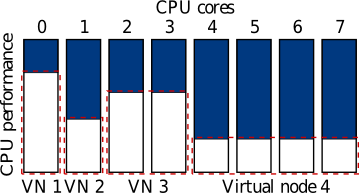
\includegraphics[scale=0.70]{Pictures/png/Distem_repartion_coeurs_v1}
  \caption{Répartition des c\oe urs d'un processeur d'une machine hôte entre les différents noeuds virtuels qu'elle héberge et émulation de leur puissance en utilisant qu'une partie de leur puissance.}
  \label{Distem_core}
\end{figure}
  
On construit ensuite l'environnement de test en plaçant les n\oe uds virtuels
sur une machine physique. Pour que l'environnement de test se rapproche au plus
près de la réalité, Distem peut changer à la volée les paramètres du réseau et
la vitesse de chaque c\oe ur alloué à un n\oe ud virtuel.

\begin{figure}
  \centering
  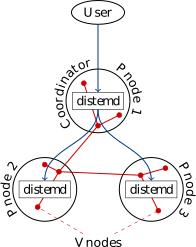
\includegraphics{Pictures/png/Distem_architecture}
  \caption{Architecture de communication de Distem. On a 3 n\oe uds physique (``Pnodes'') contenant chacun 3 n\oe uds virtuels (``Vnodes'').}
  \label{Distem_archi}
\end{figure}

Comme le présente la Figure \ref{Distem_archi}, Distem repose sur une architecture
simple pour construire son environnement de test distribué virtuel : les
``Pnodes'' et les ``Vnodes''. Les premiers sont des n\oe uds physiques non
virtualisés alors que les seconds représentent les n\oe uds que l'on souhaite
émuler. Un des Pnodes appelé ``coordinator'' gère le contrôle de
l'infrastructure dans sa globalité en communiquant avec l'ensemble des
Pnodes. Ces derniers peuvent héberger plusieurs Vnodes, chaque Pnode possèdant
son démon Distem qui les contrôle. Les Vnodes sont séparés et n'ont pas
connaissance des autres Vnodes présents sur le ``Pnode''. Pour permettre cela,
Distem utilise un conteneur LXC pour émuler un Vnode. Ainsi, chaque Vnode
possède un espace d'adressage séparé pour les ressources sytème (tâches,
interfaces réseau, mémoire...). Néanmoins, les conteneurs LXC partagent
l'utilisation du processeur, ainsi on ne peut pas attribuer un certain nombre de
c\oe urs de CPU à un Vnode. Pour pallier ce problème, Distem utilise en
parallèle le \textit{Linux Control Group{\color{red} todo définir}}. Pour
contrôler la puissance des c\oe urs attribués à chaque Vnode, Distem utilise
l'algorithme \textit{CPU-Hogs{\color{red} todo définir}}
\citep{DISTEM_buchert2011methods}. Ainsi les Vnodes ont connaissance les uns des
autres uniquement via le réseau virtuel. Chaque Vnodes possède une ou plusieurs
interfaces réseau virtuelles reliées au réseau physique de l'hôte pour pouvoir communiquer avec l'extérieur. Du fait du grand nombre de n\oe
uds qu'on souhaite émuler et qui vont communiquer entre eux cet accès au réseau
extérieur pose problème. En effet, pour se reconnaître les n\oe uds vont faire
des requêtes ARP et s'ils sont trop nombreux à envoyer ces requêtes en même
temps on va se retrouver face à un problème d'ARP flooding. La première solution
mise en place par Distem a été d'augmenter la taille des tables ARP pour les
Pnodes et les Vnodes ainsi que l'augmentation du \textit{timeout} d'une entrée
dans la table. Néanmoins, le but de Distem étant de pouvoir émuler de plus en
plus de n\oe uds cette solution finira par ne plus pouvoir s'appliquer. Une
autre solution, qui est celle utilisée actuellement, est de rajouter une couche
d'abstraction réseau à l'intérieur du Pnode en utilisant
VXLAN\citep{VXLAN_mahalingam2014virtual, DISTEM_buchert2014emulation} comme le
montre la Fig.\ref{Distem_VXLAN}. Ainsi, les paquets seront échangés entre
Pnodes sur le réseau et c'est la couche VXLAN qui s'occupera d'envoyer au bon
Vnodes le paquet reçu sur le Pnodes. Ces derniers étant très peu nombreux on est
sûrs de ne pas surcharger les tables ARP.

\begin{figure}[H]
  \centering
  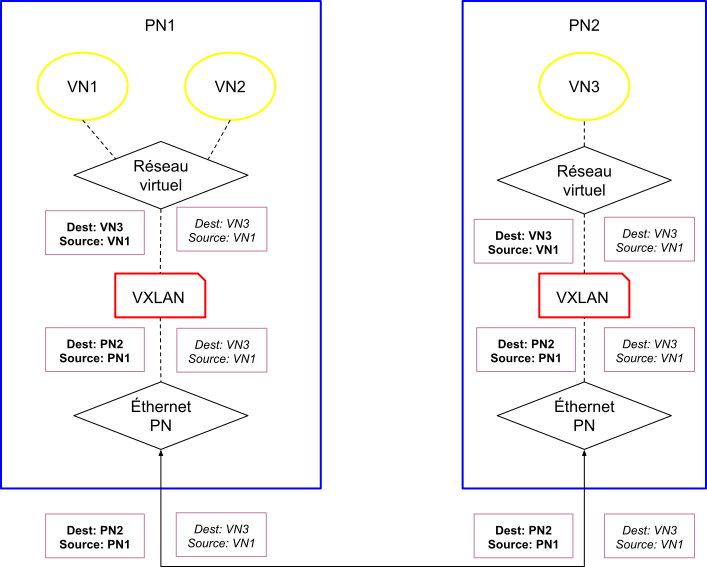
\includegraphics[scale=0.45]{Pictures/png/Distem_VXLAN}
  \caption{Abstractions des communications réseaux de Distem via VXLAN. Les paquets en gras sont ceux envoyés en présence de VXLAN et ceux en italiques sont ceux qui seraient envoyés sur un réseau n'utilisant pas VXLAN.}
  \label{Distem_VXLAN}
\end{figure}

On voit donc que Distem possède une infrastructure et un réseau émulé bien
détaillés et assez réalistes. De plus il est capable de gérer les fautes
injectées au niveau des n\oe uds ou sur le réseau. Son seul problème est donc d'utiliser la virtualisation par limitation empêchant ainsi l'émulation de machines plus rapides.
